\documentclass[border=3pt]{standalone}
% Preâmbulo compartilhado pelos diagramas TikZ da aula 12 (Mapeamento por Grade de Ocupação)
\usepackage[T1]{fontenc}
\usepackage[utf8]{inputenc}
\usepackage{lmodern}
\usepackage{amsmath}
\usepackage{xcolor}
\usepackage{tikz}
\usetikzlibrary{arrows.meta,angles,quotes,decorations.pathmorphing,calc,
                positioning,shapes.geometric,shapes.misc,backgrounds,fit,
                math}

% Paleta (mesma dos SVGs originais)
\definecolor{dblue}{HTML}{2A5B8C}
\definecolor{dorange}{HTML}{B3541E}
\definecolor{dgreen}{HTML}{4A7C59}
\definecolor{dred}{HTML}{9C4B4B}
\definecolor{dcream}{HTML}{F4F1EA}
\definecolor{dshade}{HTML}{DDD7C9}

% Função gaussiana (não normalizada por padrão de escala visual)
\pgfmathdeclarefunction{gauss}{3}{%
  \pgfmathparse{1/(#3*sqrt(2*pi))*exp(-((#1-#2)^2)/(2*#3^2))}%
}

% Estilos comuns (prefixo d... para não colidir com chaves internas do pgf)
\tikzset{
  >={Stealth[length=2mm]},
  dguide/.style={gray!55, dashed, line width=0.4pt},
  daxis/.style={gray!60, line width=0.7pt, ->},
  dbody/.style={fill=black!3, draw=black!80, line width=1pt},
  dacc/.style={draw=dblue, line width=1pt},
  dlbl/.style={black!55, font=\small},
  dsub/.style={black!45, font=\footnotesize},
  dstate/.style={circle, draw=black!80, fill=dcream, line width=1pt,
                 minimum size=17mm, font=\large, inner sep=1pt},
  dobs/.style={circle, draw=black!80, fill=dshade, line width=1pt,
               minimum size=14mm, font=\large, inner sep=1pt},
  dbox/.style={rounded corners=2pt, draw=black!80, fill=dcream, line width=1pt,
               align=center, inner sep=6pt},
  dop/.style={circle, draw=black!80, fill=white, line width=1pt,
              minimum size=6mm, inner sep=0pt, font=\small},
  dtrans/.style={->, dblue, line width=1pt},
  dmeas/.style={->, dorange, line width=1pt},
  dcurve/.style={line width=1pt, dblue},
  dcurveb/.style={line width=1.4pt, dorange},
}

\begin{document}
\hyphenpenalty=10000 \exhyphenpenalty=10000 \tolerance=9999 \emergencystretch=3em
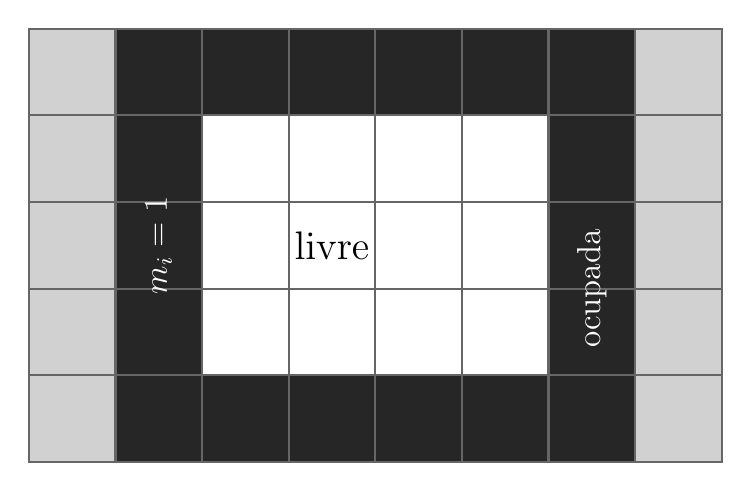
\begin{tikzpicture}[x=1cm,y=1cm]
  \tikzset{c0/.style={fill=white, draw=black!60, line width=0.8pt}, c1/.style={fill=black!85, draw=black!60, line width=0.8pt}, cx/.style={fill=black!18, draw=black!60, line width=0.8pt}}
  \foreach \x in {0,...,7} {\foreach \y in {0,...,4} {\draw[cx] (\x*1.1,\y*1.1) rectangle +(1.1,1.1);}}
  \foreach \x/\y in {1/4, 2/4, 3/4, 4/4, 5/4, 6/4, 1/0, 2/0, 3/0, 4/0, 5/0, 6/0, 1/1, 1/2, 1/3, 6/1, 6/2, 6/3} {\draw[c1] (\x*1.1,\y*1.1) rectangle +(1.1,1.1);}
  \foreach \x/\y in {2/1, 3/1, 4/1, 5/1, 2/2, 3/2, 4/2, 5/2, 2/3, 3/3, 4/3, 5/3} {\draw[c0] (\x*1.1,\y*1.1) rectangle +(1.1,1.1);}
  \node[font=\Large] at (3.85,2.75) {livre};
  \node[font=\large, white, rotate=90] at (1.65,2.75) {$m_i=1$};
  \node[font=\large, white, rotate=90] at (7.15,2.2) {ocupada};
\end{tikzpicture}
\end{document}
